\chapter{HARDWARE IMPLEMENTATION}\label{chap-hardware}
\thispagestyle{empty}

This chapter presents the practical implementation of the proposed cold plasma generation system. The hardware development followed an iterative approach, beginning with a perfboard prototype for initial validation, followed by multiple PCB design iterations to achieve a stable and reliable system. The final implementation includes the inverter, gate driver, power supply, controller, sensing modules, transformer, and voltage multiplier.

\section{Perfboard Prototype}

A full-bridge inverter prototype using IRFP460 MOSFETs and the UCC21330 gate driver was initially implemented on a perfboard for functional validation.

This prototype verified correct circuit operation and confirmed the validity of the schematic design. During testing, it was observed that the bootstrap resistor required a higher power rating than 1/4 W, as lower-rated resistors overheated under operating conditions. This stage enabled validation of component selection and system functionality prior to PCB implementation.

\begin{figure}[H]
\centering
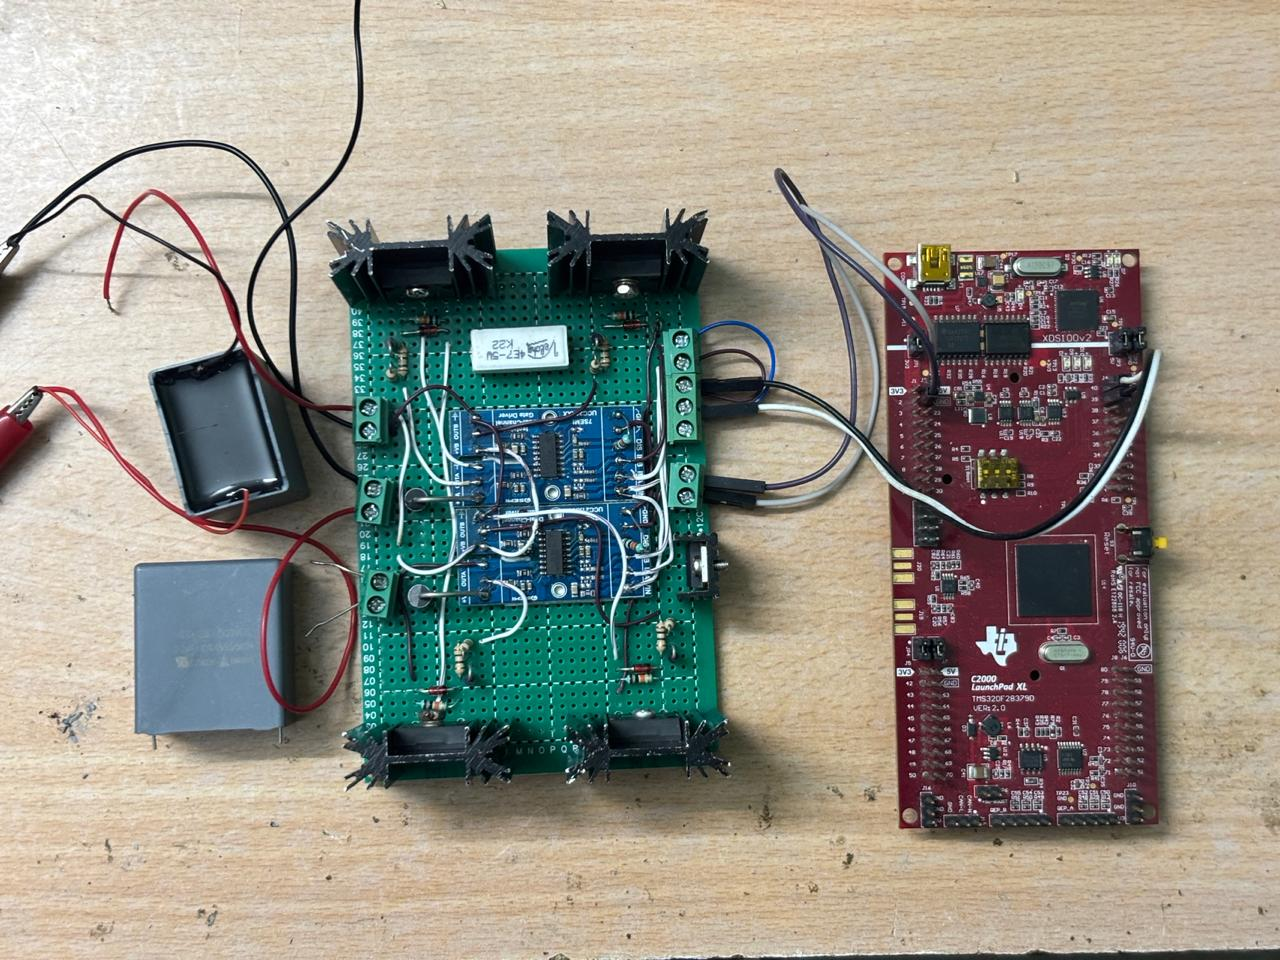
\includegraphics[width=.75\linewidth]{./picture-files/perfboard_hbridge.jpg}
\caption{Perfboard implementation of the H-Bridge and UCC21330 gate driver for initial testing with LAUNCHXL F28379D Microcontroller.}
\label{fig:perfboard}
\end{figure}

\section{Initial PCB Design}

Based on the validated prototype, an initial PCB design was developed consisting of a plug-in UCC21330 gate driver module and a separate H-bridge board.

During high-voltage testing, a critical design flaw was identified: the grounds of the isolated sections of the UCC21330 were inadvertently connected. This violated the isolation requirement of the driver and resulted in failure of multiple driver ICs.

\begin{figure}[H]
\centering

\begin{subfigure}[b]{0.48\textwidth}
    \centering
    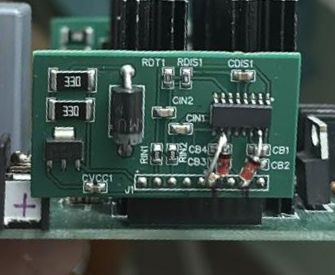
\includegraphics[width=\textwidth]{./picture-files/old_h_bridge/uccdriver.jpeg}
    \caption{Gate driver board using UCC21330}
    \label{fig:gatedriver}
\end{subfigure}
\hfill
\begin{subfigure}[b]{0.48\textwidth}
    \centering
    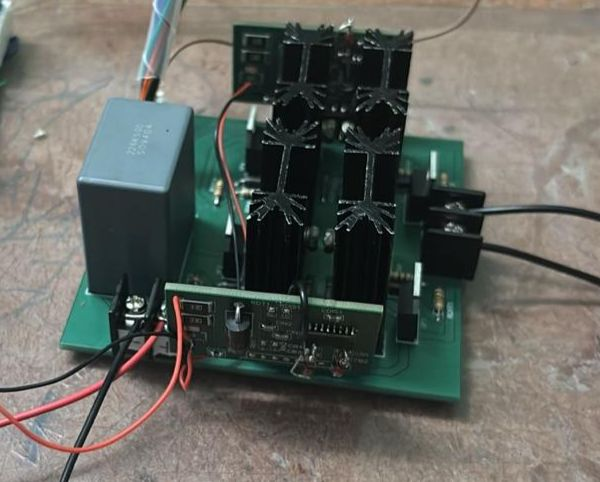
\includegraphics[width=\textwidth]{./picture-files/old_h_bridge/fullbridge.jpeg}
    \caption{H-Bridge circuit board}
    \label{fig:initial-pcbs}
\end{subfigure}

\caption{Initial PCB implementation.}
\label{fig:overall}
\end{figure}



\section{Final PCB Implementation}

The final PCB design was developed by addressing the issues identified in earlier iterations.

The following improvements were implemented:

\begin{itemize}
    \item Proper isolation between high-side and low-side grounds of the UCC21330  
    \item Optimized PCB layout to reduce parasitic inductance and switching noise  
    \item Reduced ringing through improved trace routing and compact design  
    \item Addition of electrolytic and film capacitors for effective decoupling and high-frequency noise suppression  
\end{itemize}

\begin{figure}[H]
\centering

\begin{subfigure}[t]{0.48\textwidth}
    \centering
    
\includegraphics[width=\textwidth]{./picture-files/UCC21330_DRIVER/PCB_IMAGE_1.jpeg}
    \caption{Gate driver board using UCC21330}
    \label{fig:gatedriver2}
\end{subfigure}
\hfill
\begin{subfigure}[t]{0.48\textwidth}
    \centering
    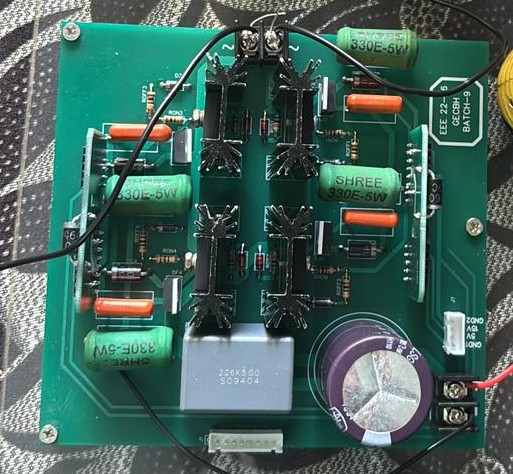
\includegraphics[width=\textwidth]{./picture-files/NEW_H_BRIDGE_DRIVER/PCB_IMAGE_1.jpeg}
    \caption{H-Bridge PCB board}
    \label{fig:finaal-pcbs}
\end{subfigure}

\caption{Final PCB implementation with improved layout and filtering.}
\label{fig:overall}
\end{figure}

These modifications resulted in improved stability and reliable operation at higher voltages.
\newpage

\section{Power Supply Board}

The power supply board provides the required DC voltage levels for different subsystems. The input is 230 V AC, which is rectified to generate approximately 320 V DC for the inverter stage, along with regulated 12 V and 5 V supplies for the gate driver and microcontroller respectively.

The board was fabricated using a PCB etching process and tested prior to system integration. The 5 V supply is provided by the Hi-Link HLK-10M05 module, while the 12 V supply is generated using the Hi-Link HLK-10M12 module. The 320 V DC link is obtained through a rectifier stage, as detailed in Section \ref{subsec:powerdesign}.

\begin{figure}[H]
\centering

\includegraphics[width=0.65\linewidth]{./picture-files/PowerSupplyBoard/PCB_IMAGE_1.jpeg}
\caption{Etched PCB of Power Supply Board.}
\label{fig:final-pcbs}
\end{figure}

\begin{figure}[H]
\centering
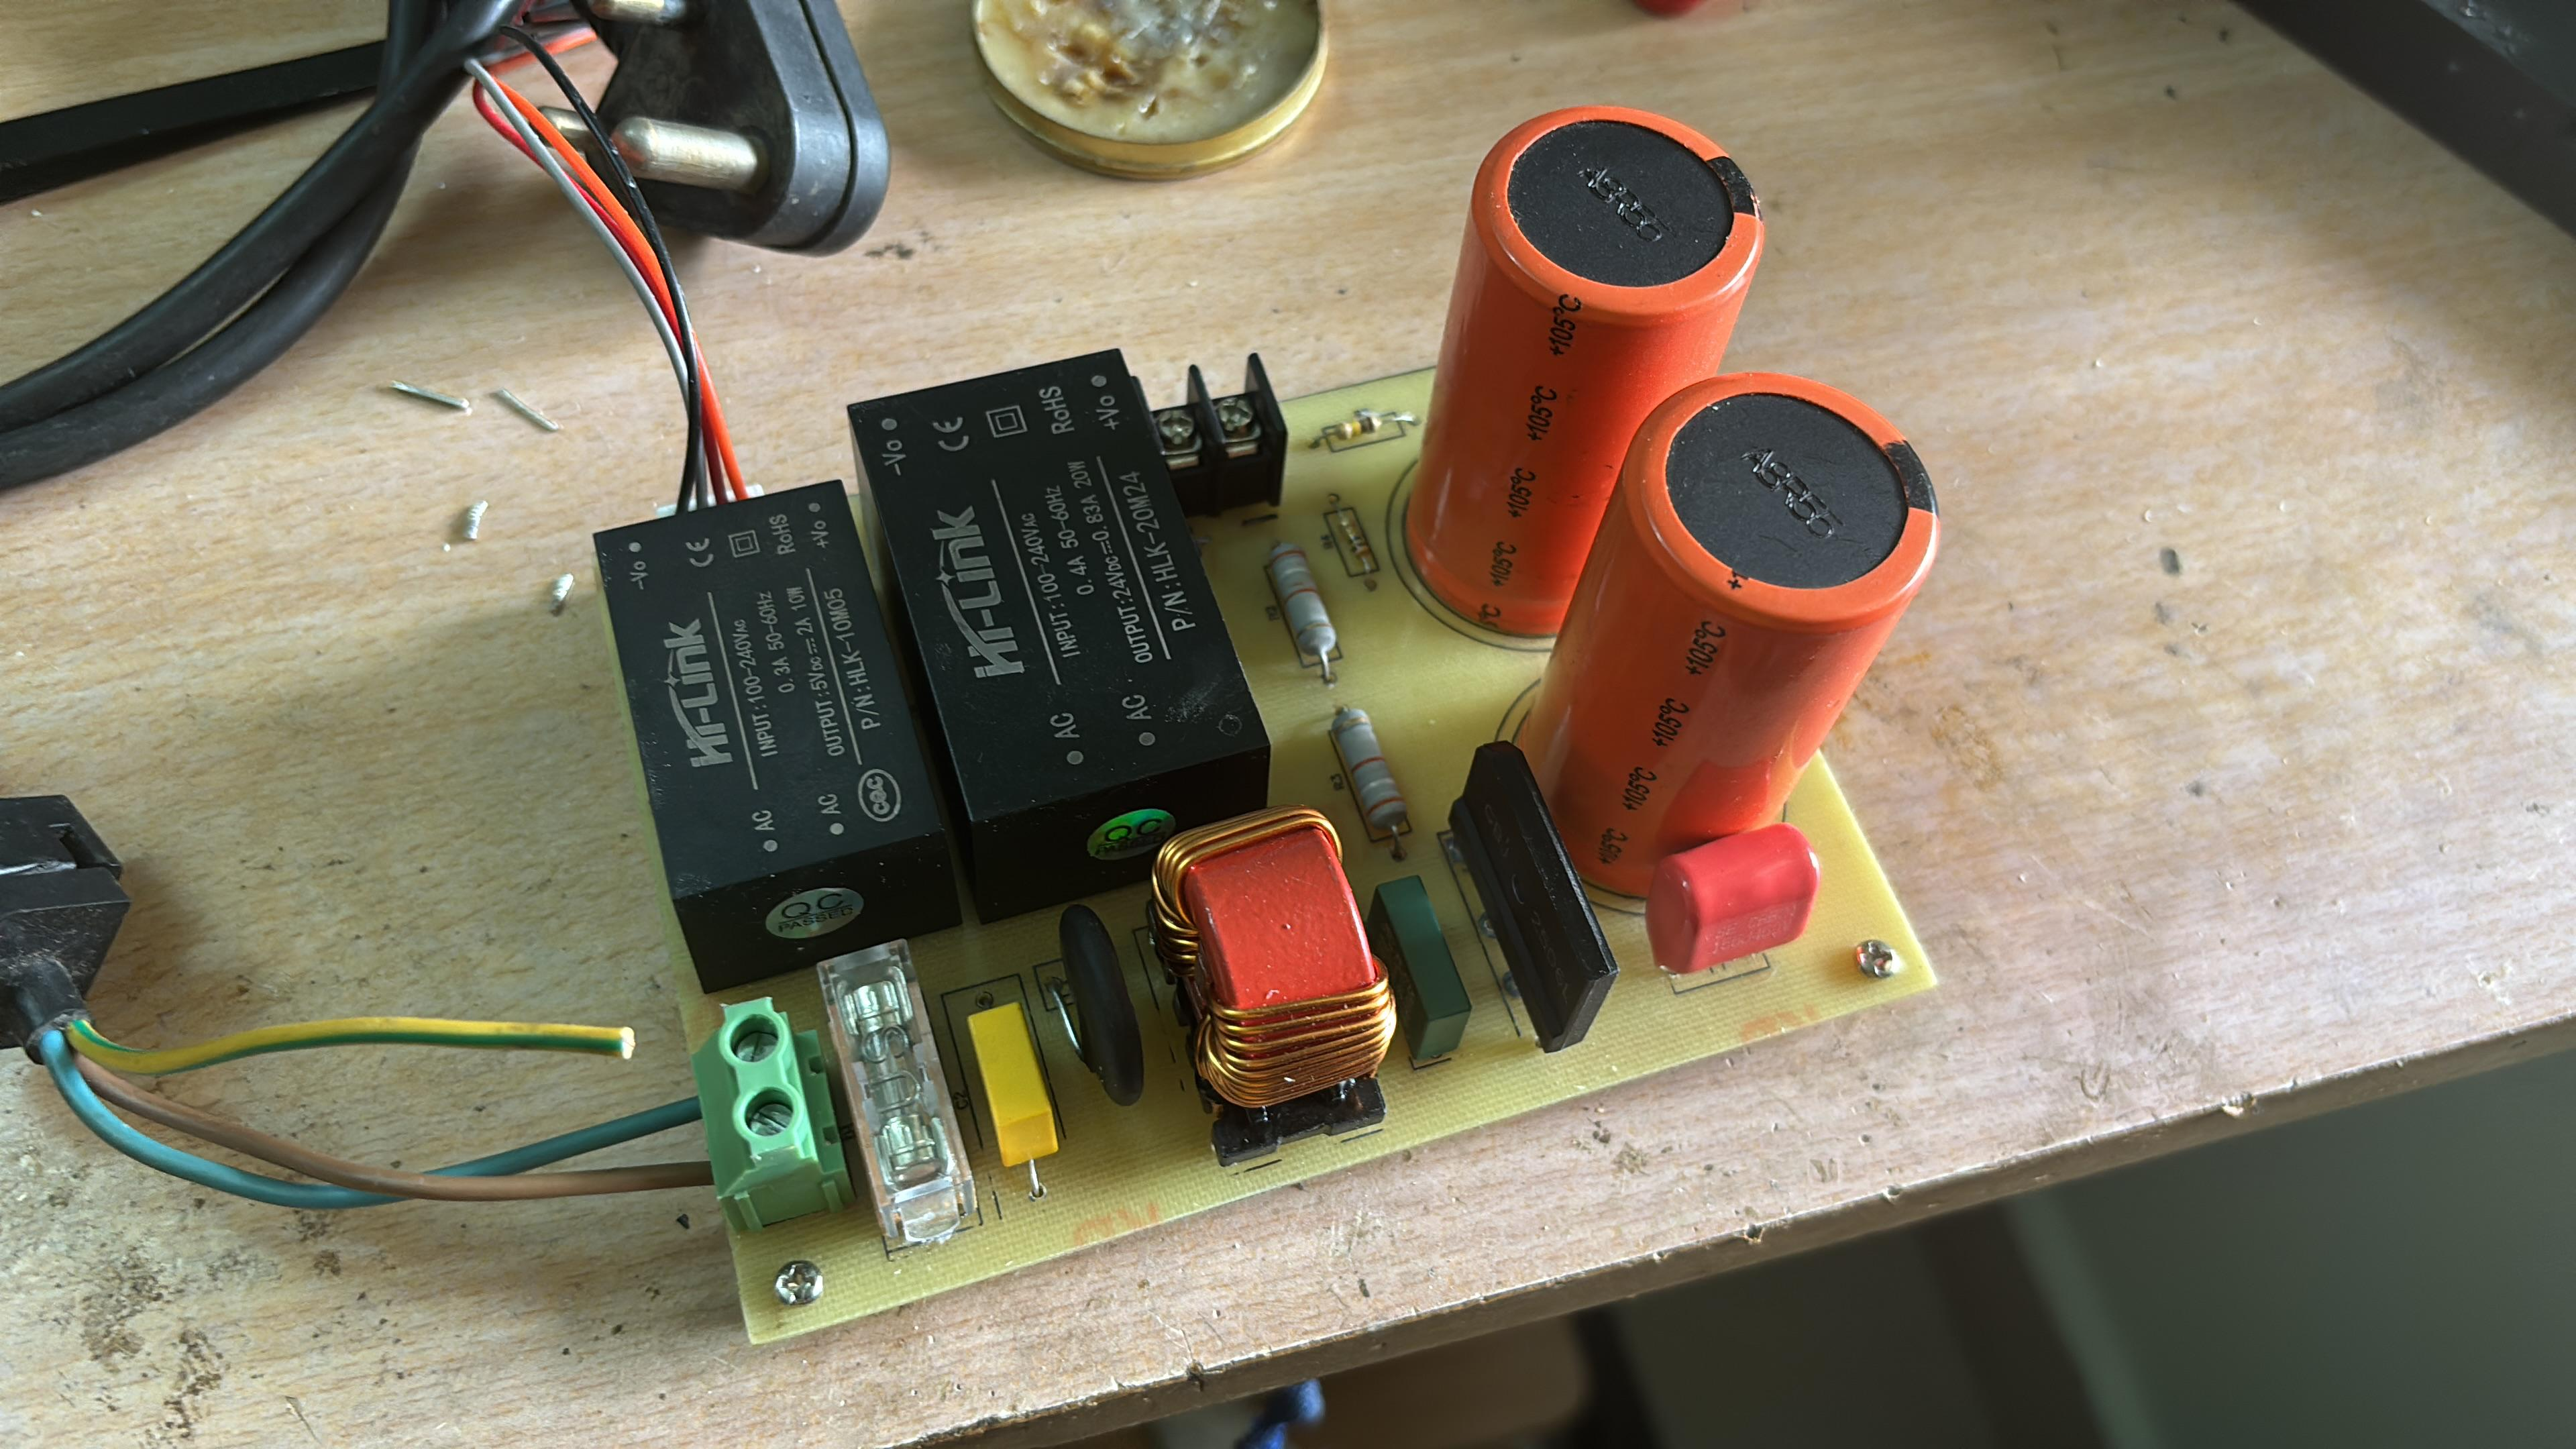
\includegraphics[width=0.75\linewidth]{./picture-files/PowerSupplyBoard/Full Board.jpeg}
\caption{PCB implementation of Power Supply Board.}
\label{fig:final-pcbs}
\end{figure}

\section{H-Bridge Inverter}

The H-bridge inverter converts the DC link voltage into a high-frequency AC signal required to drive the transformer.

It is implemented using four IRFP460 MOSFETs driven by the UCC21330 gate driver. The inverter operates at approximately 100 kHz, generating a square wave output at the transformer primary. Heat sinks are used to dissipate thermal losses during operation.

Oscilloscope measurements confirmed correct switching behavior and proper waveform generation.

\begin{figure}[H]
\centering
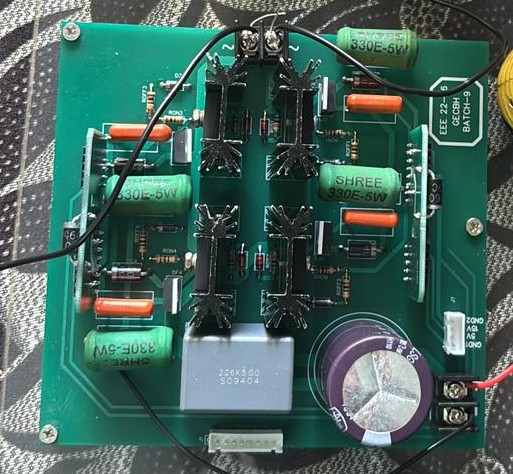
\includegraphics[width=0.7\linewidth]{./picture-files/NEW_H_BRIDGE_DRIVER/PCB_IMAGE_1.jpeg}
\caption{Final PCB implementation of H-Bridge.}
\label{fig:final-pcbs}
\end{figure}

\section{Controller Board}

The system is controlled using an STM32G431 microcontroller.

The controller performs the following functions:

\begin{itemize}
    \item Generates complementary PWM signals with adjustable phase shift for inverter control  
    \item Acquires voltage and current feedback using ADC  
    \item Displays measured values on an LCD  
    \item Implements overcurrent protection by disabling the gate driver when current exceeds 1.5 A  
\end{itemize}

\begin{figure}[H]
\centering
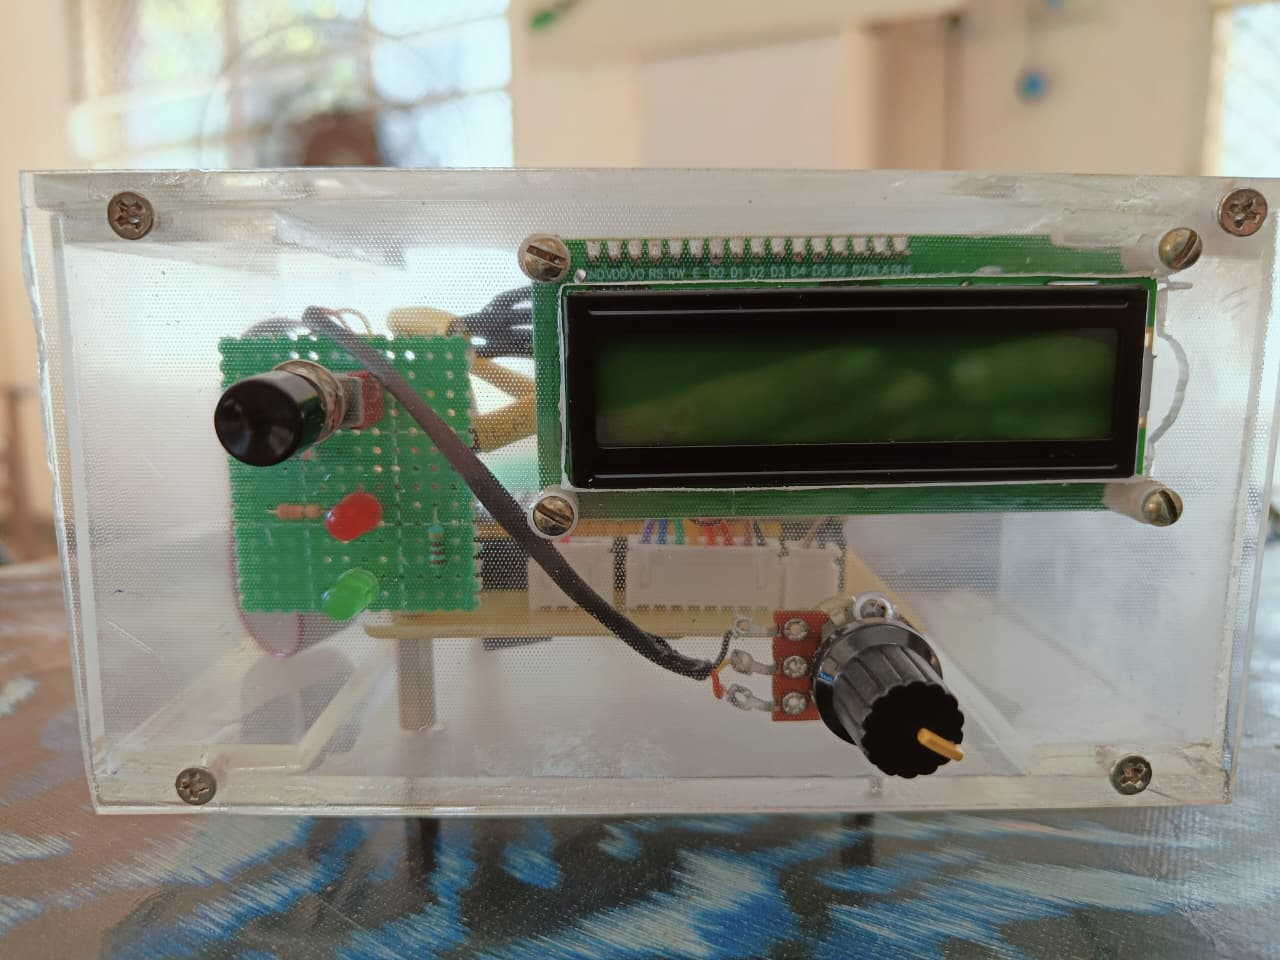
\includegraphics[width=0.8\linewidth]{./picture-files/controllerboard.jpeg}
\caption{Controller Board.}
\label{fig:final-pcbs}
\end{figure}

\section{Voltage and Current Sensor Circuit}

The sensing module monitors DC bus voltage and load current during operation. The STM32 uses a 12-bit ADC (0–3.3 V input range) to digitize these signals.

Calibration was performed using standard instruments over the following ranges:

\begin{itemize}
    \item Current: 0–3 A  
    \item Voltage: 20–350 V  
\end{itemize}

Measured ADC values were scaled and used to derive calibration relationships between digital readings and actual values.

\begin{figure}[H]
\centering
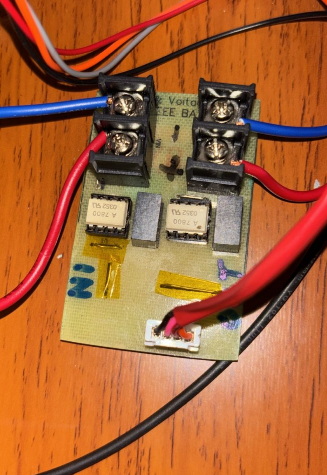
\includegraphics[width=0.45\linewidth]{./picture-files/Sensors/sensorpic.png}
\caption{Final PCB implementation of Voltage and Current Sensors.}
\label{fig:final-pcbs}
\end{figure}

\section{Transformer Fabrication}

A high-frequency step-up transformer was designed using an ETD-59 ferrite core for operation at 100 kHz.

The transformer consists of:
\begin{itemize}
    \item Primary winding: 14 turns  
    \item Secondary winding: 170 turns  
\end{itemize}

To reduce skin effect losses, the primary winding uses multiple parallel strands of copper wire. The windings were arranged on a 3D-printed bobbin, with primary winding placed internally and secondary winding externally.

To improve insulation and reduce capacitive coupling, the core was wrapped with insulating tape followed by a grounded copper shield. The assembled transformer was tested to verify voltage step-up performance and thermal stability.

\begin{figure}[H]
\centering
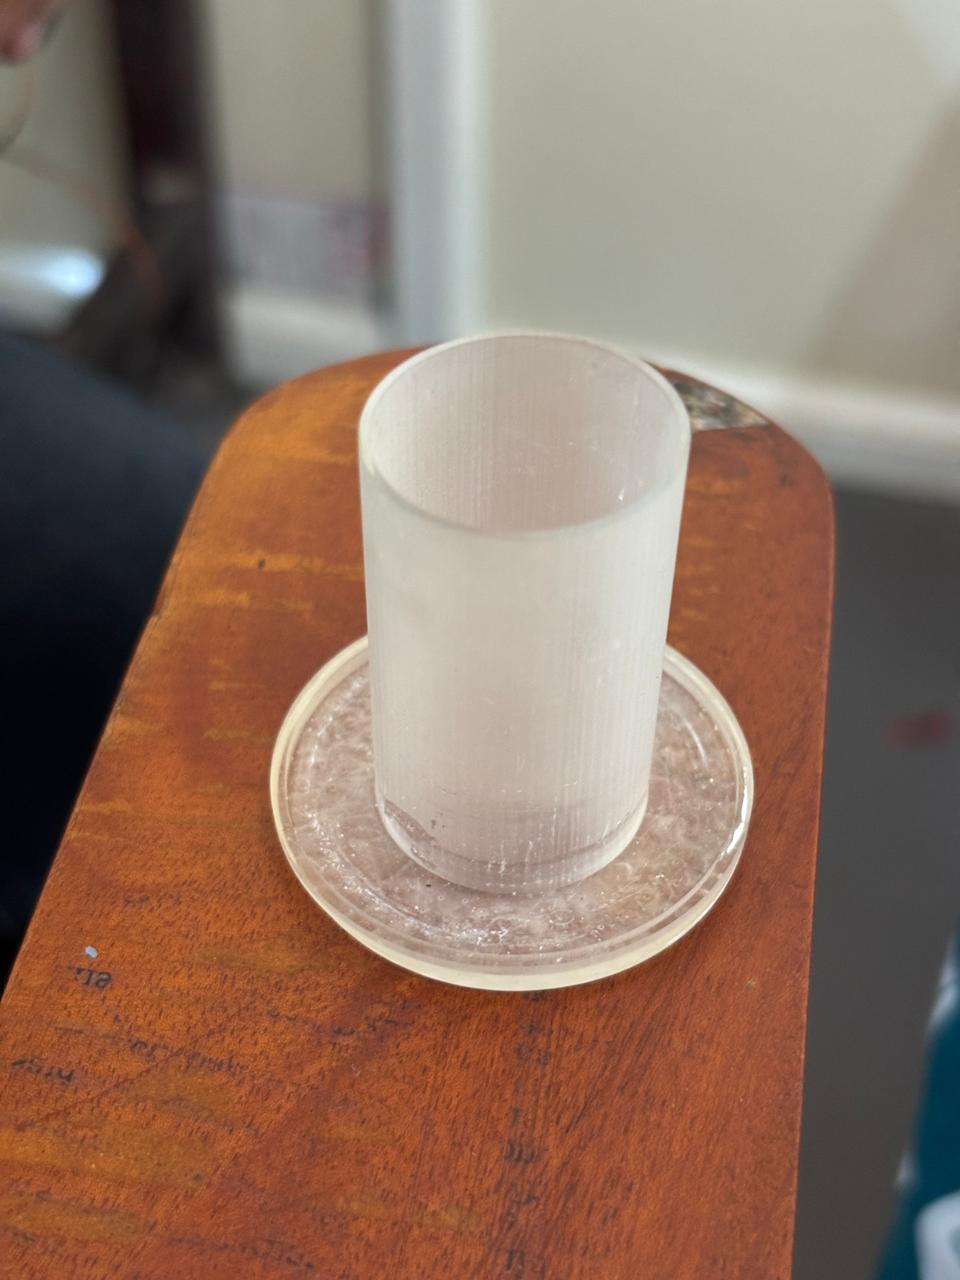
\includegraphics[width=0.325\textwidth]{./picture-files/Transformer New/Inner Piece.jpeg}
\hfill
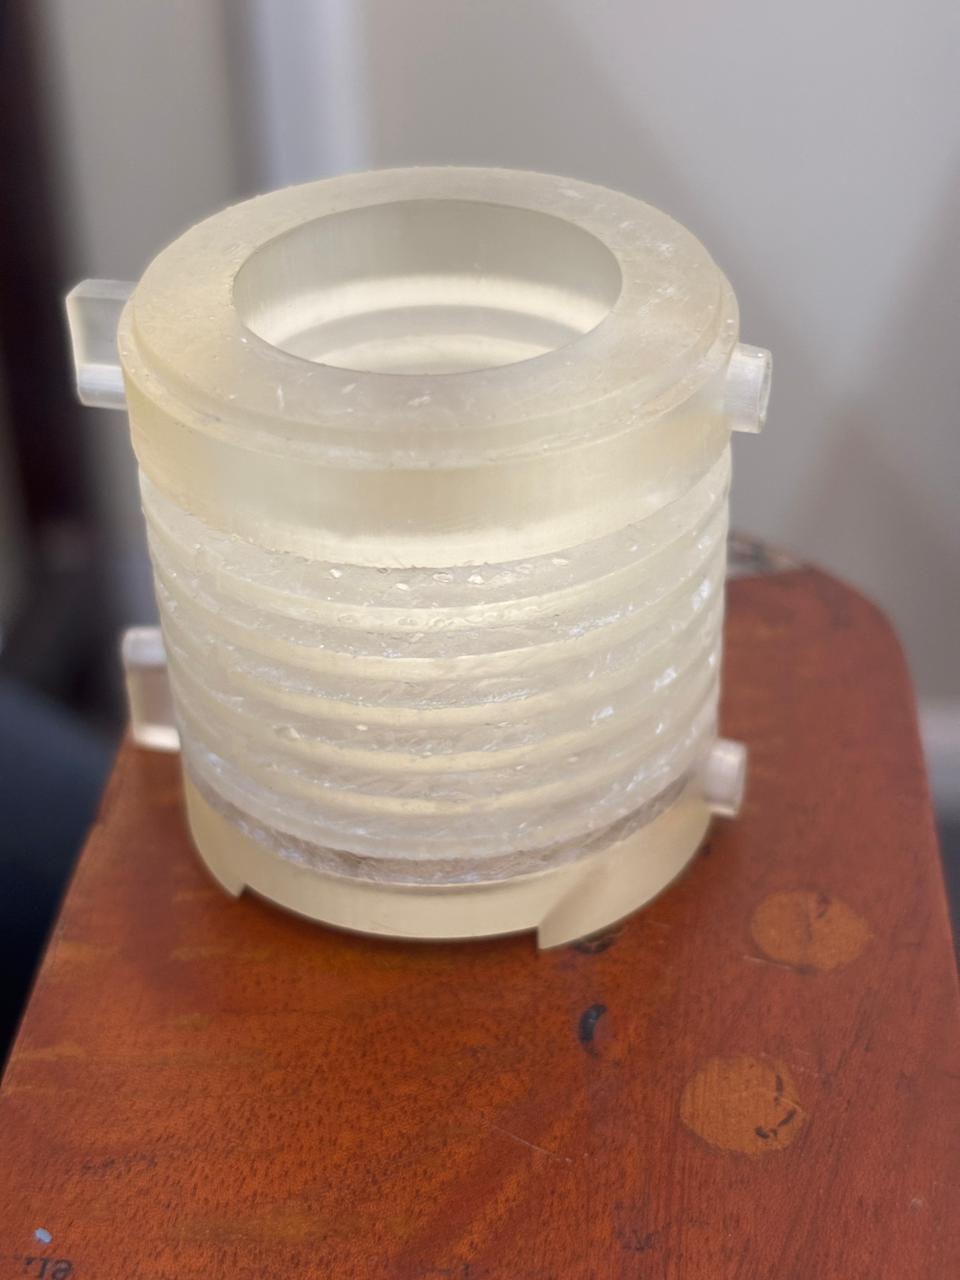
\includegraphics[width=0.325\textwidth]{./picture-files/Transformer New/Outer Piece.jpeg}
\hfill
\includegraphics[width=0.325\textwidth]{./picture-files/Transformer New/Secondary windings.jpeg}
\caption{Inner and outer parts of bobbin and secondary windings.}
\label{fig:transformerbobin}
\end{figure}

\begin{figure}[H]
\centering
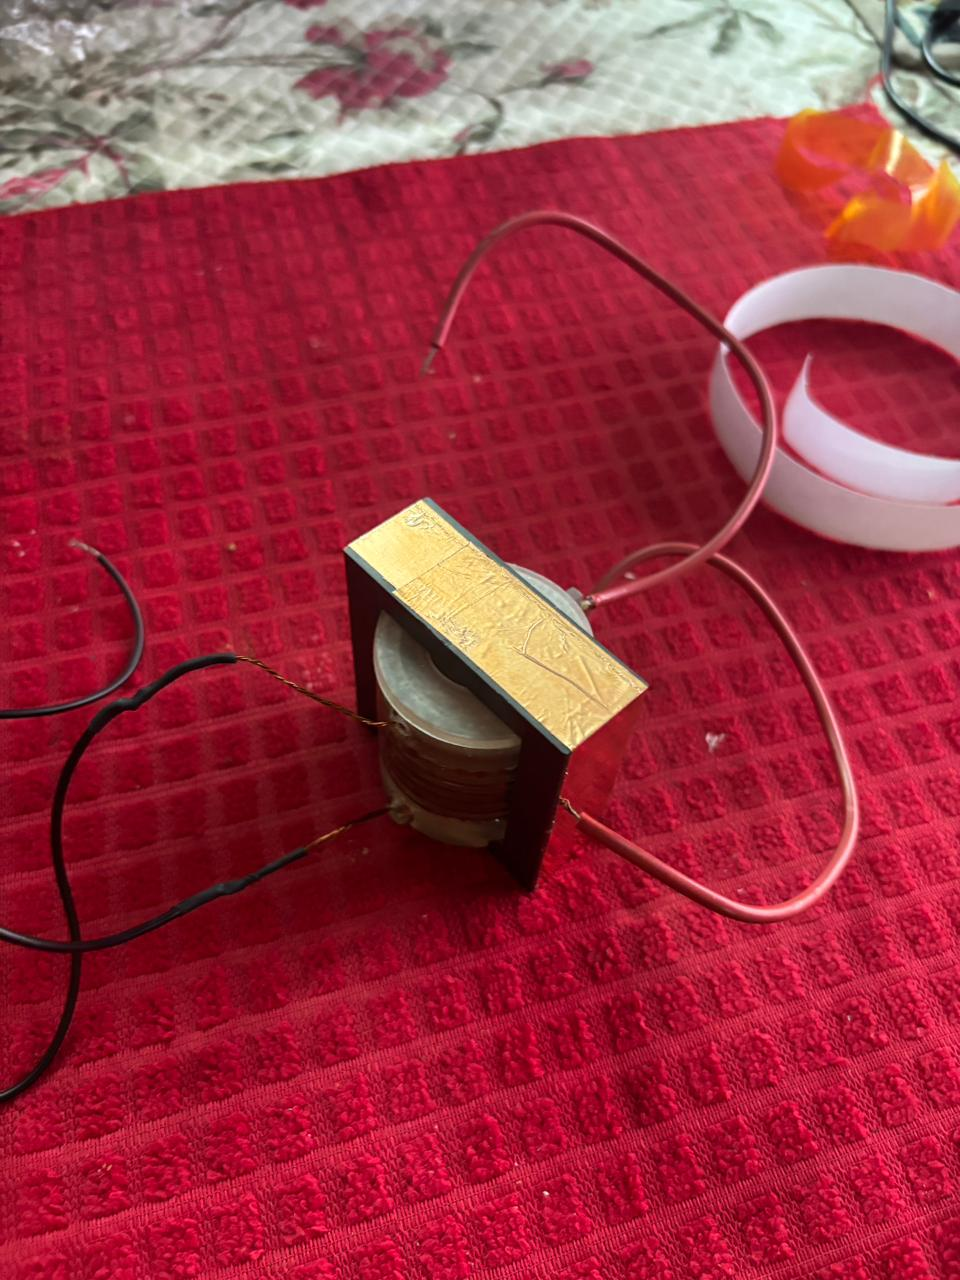
\includegraphics[width=0.35\linewidth]{./picture-files/Transformer New/Ground Sheeted.jpeg}
\includegraphics[width=0.55\linewidth]{./picture-files/Transformer New/assembled.jpeg}
\caption{Ground shielding and final transformer assembly.}
\label{fig:wounded transformer}
\end{figure}

\section{Cockcroft--Walton Voltage Multiplier}

The Cockcroft–Walton voltage multiplier is used to convert the transformer output (approximately 4 kV AC) into high-voltage DC (approximately 30 kV).

The circuit consists of cascaded diode-capacitor stages that incrementally increase the voltage. To prevent corona discharge, arcing, and surface leakage, the entire multiplier assembly is encapsulated in resin.

\begin{figure}[h!]
\centering
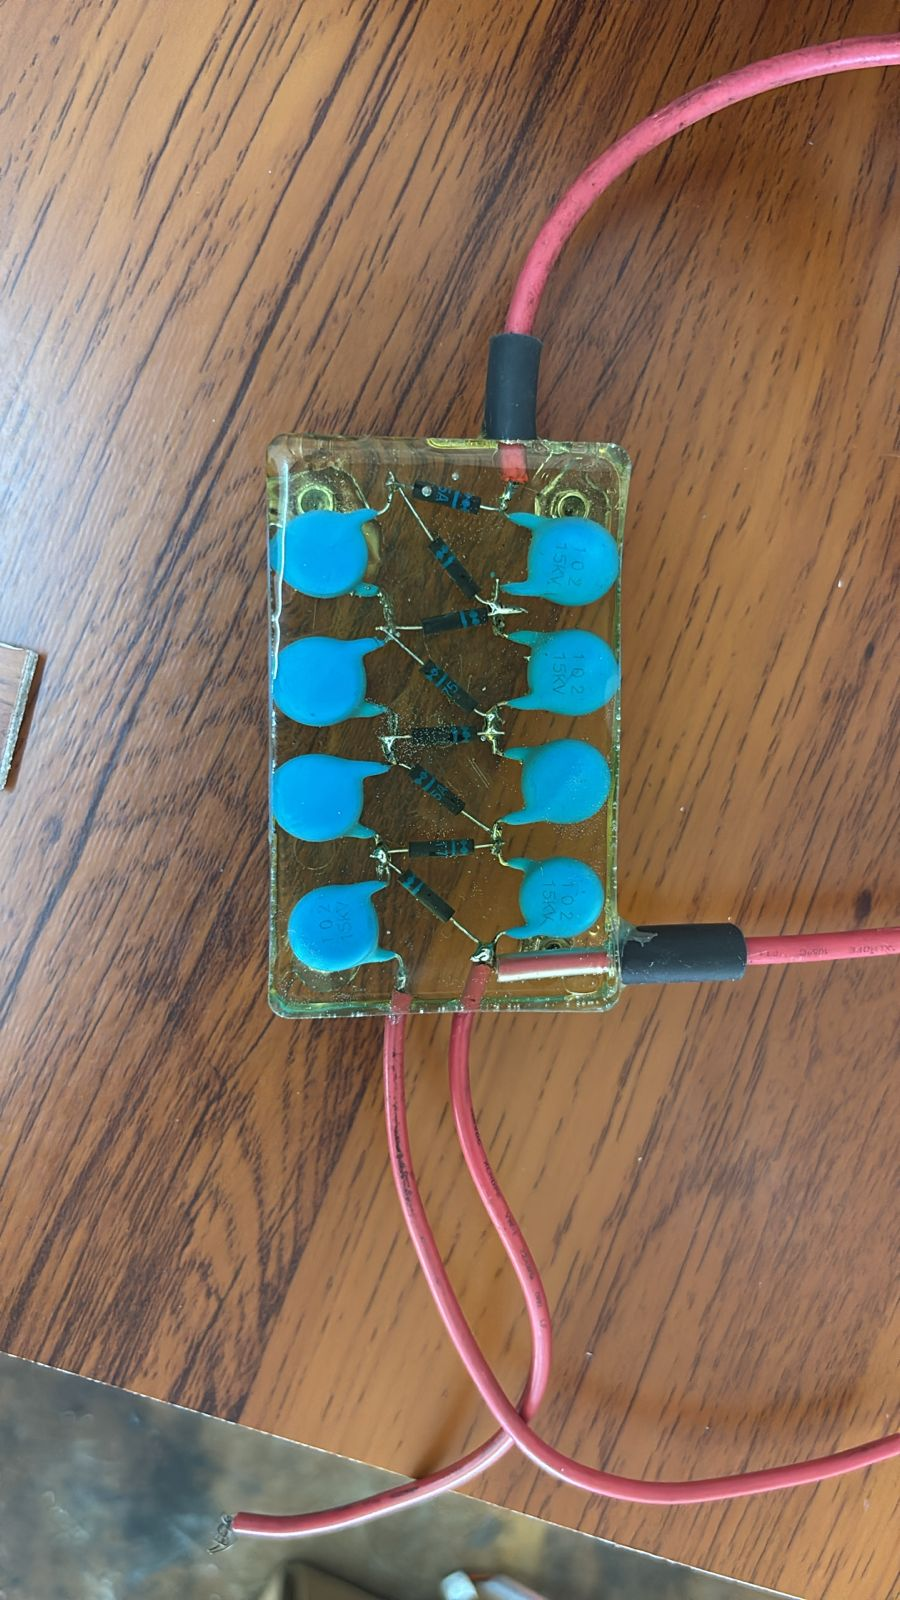
\includegraphics[width=0.45\linewidth, angle =90]{./picture-files/cockcroft-walton/voltage multiplier.jpeg}
\caption{Cockcroft-Walton Voltage Multiplier.}
\label{fig:final-pcbs}
\end{figure}

\newpage



\section{Plasma Generation Hardware Setup}

The plasma generation system consists of three primary subsystems: the argon gas supply, flow control unit, and dielectric discharge chamber.

\paragraph{Gas Supply and Flow Control}

Argon gas is stored in a \textbf{1.5 m$^3$ capacity cylinder}. The cylinder is equipped with pressure regulators, control valves, and dual pressure gauges to monitor cylinder pressure and regulated outlet pressure. A calibrated flow meter is used to precisely control the gas flow rate.

The regulated gas output is delivered to the discharge setup through flexible pipes of \textbf{10 mm diameter}.

\paragraph{Discharge Chamber Configuration}

The gas line is connected to the central port of a \textbf{T-joint}. The T-joint serves as the interface between the gas flow path and the electrode assembly.

\begin{itemize}
    \item One branch of the T-joint is connected to a \textbf{glass dropper}, which functions as the dielectric discharge tube.
    \item The second branch is used to insert the \textbf{high-voltage electrode} into the glass tube.
\end{itemize}

The electrode is aligned along the axis of the dropper to establish a strong electric field concentration at the tip.

Additionally, a \textbf{ground ring electrode} is placed around a small section of the glass dropper near the outlet. This configuration enhances the electric field distribution and stabilizes the plasma discharge by forming a localized discharge region.

\paragraph{Plasma Generation}

When high voltage is applied, the flowing argon gas undergoes ionization within the electric field region. A stable plasma jet is generated at the narrow end of the glass dropper.

The discharge emerges as a directed plasma plume from the tip, with its characteristics governed by the applied voltage and gas flow rate.

\paragraph{Sealing and Mechanical Support}

All joints and connections in the setup are made \textbf{airtight} to prevent gas leakage. This ensures that the gas exits exclusively through the dropper tip, thereby improving discharge stability and efficiency.

The entire T-joint assembly and discharge structure are mounted on an \textbf{acrylic support frame}, providing mechanical rigidity and electrical insulation during operation.



\begin{figure}[H]
\centering

% First image (full width)
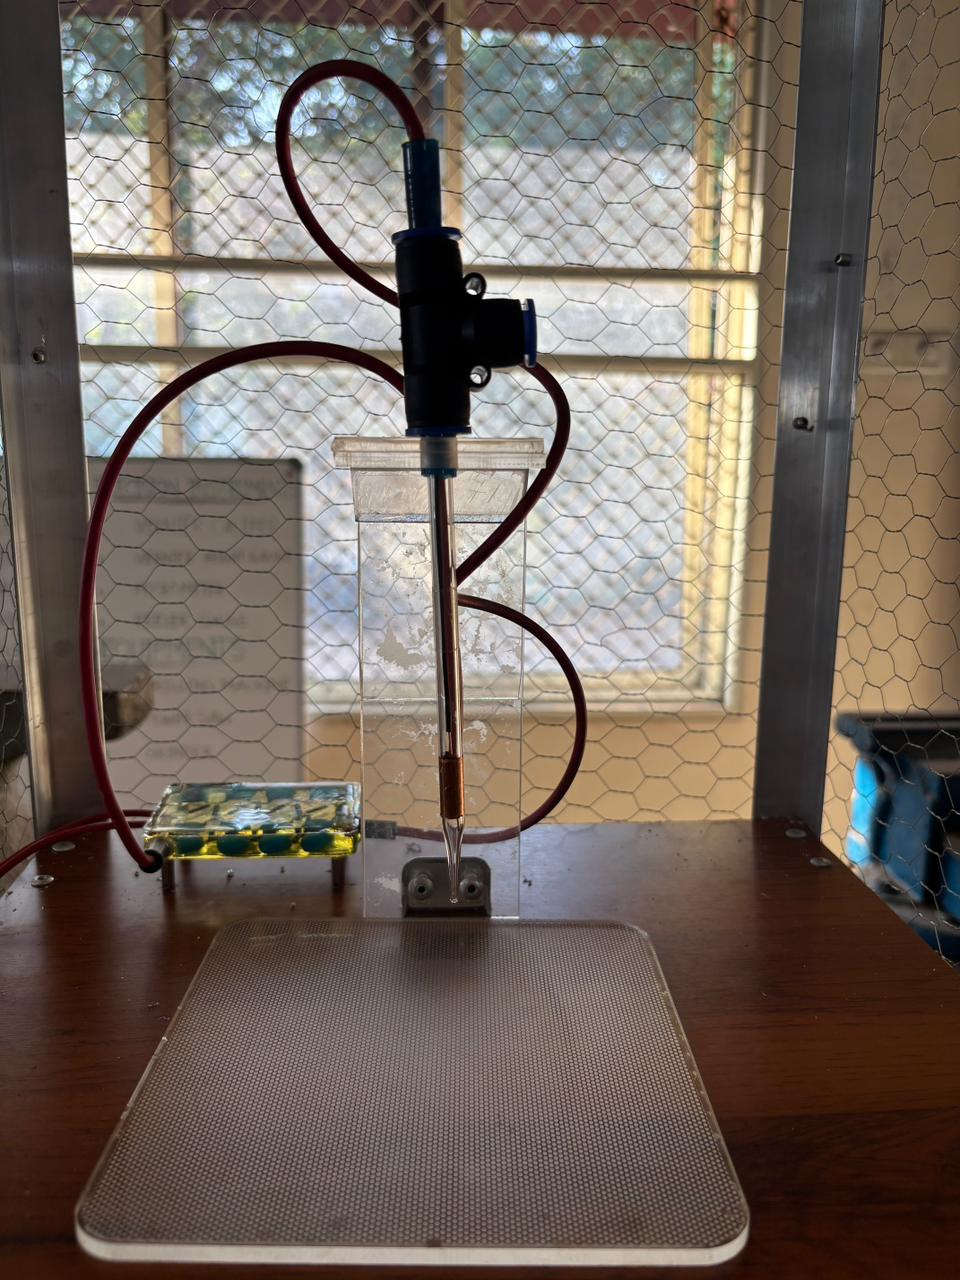
\includegraphics[width=0.75\textwidth]{./picture-files/Hardware setup/reaction chamber.jpeg}
\caption{Reaction chamber and electrode assembly}
\label{fig:reaction_chamber}

\end{figure}

\begin{figure}[H]
\centering

% Second and third images side by side
\begin{subfigure}[t]{0.44\textwidth}
    \centering
    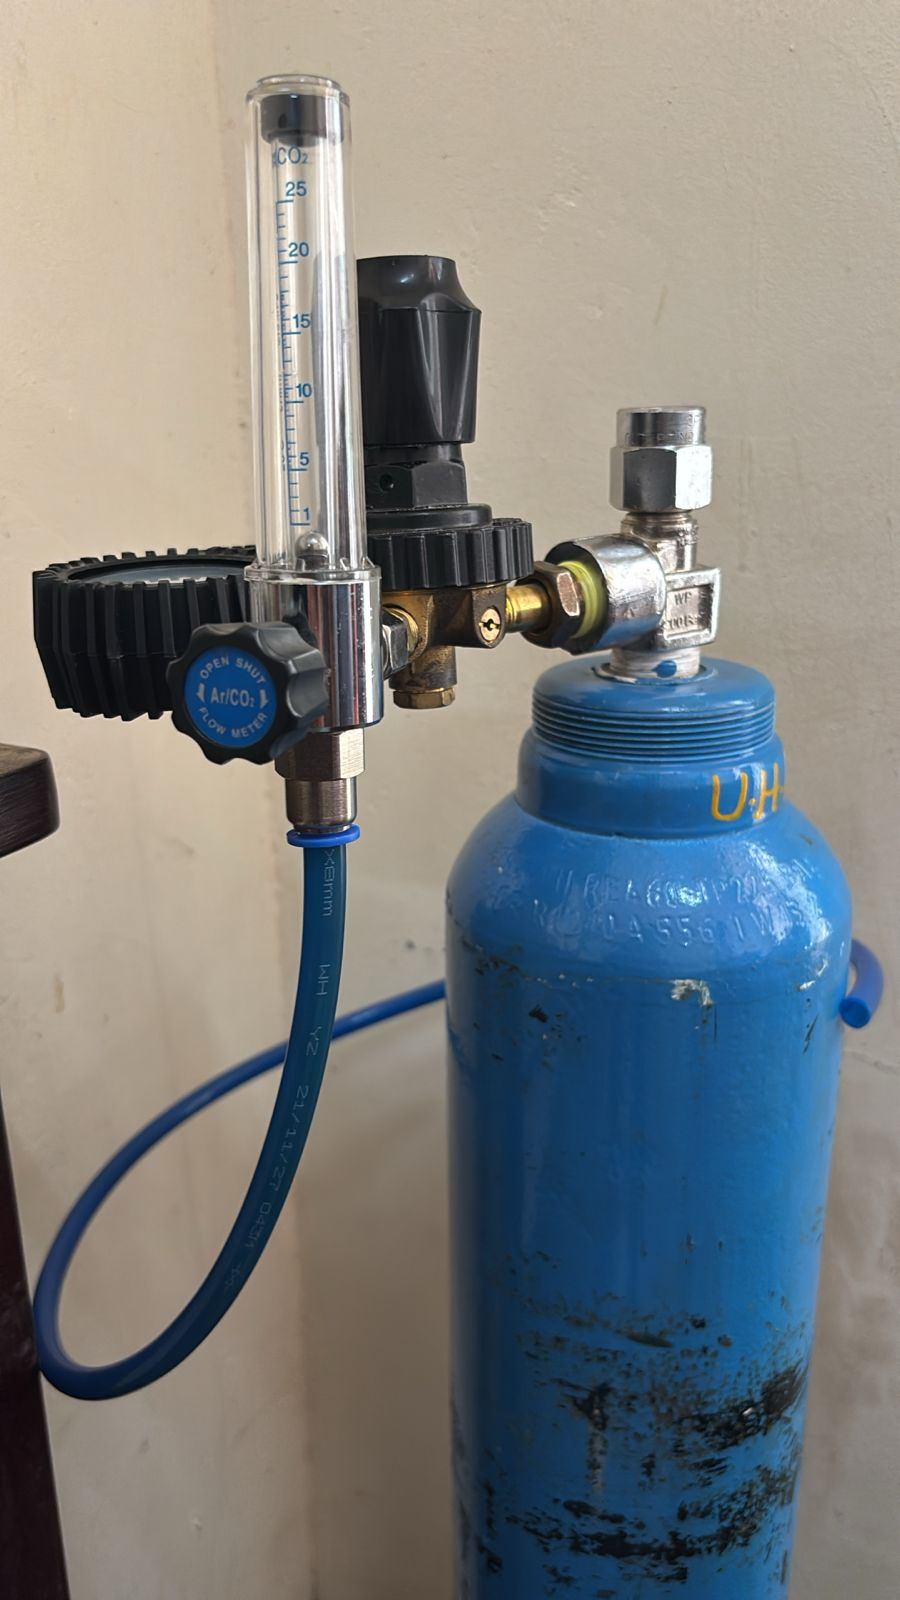
\includegraphics[width=\textwidth]{./picture-files/Hardware setup/side view.jpeg}
    \caption{Side view of the setup}
\end{subfigure}
\hfill
\begin{subfigure}[t]{0.48\textwidth}
    \centering
    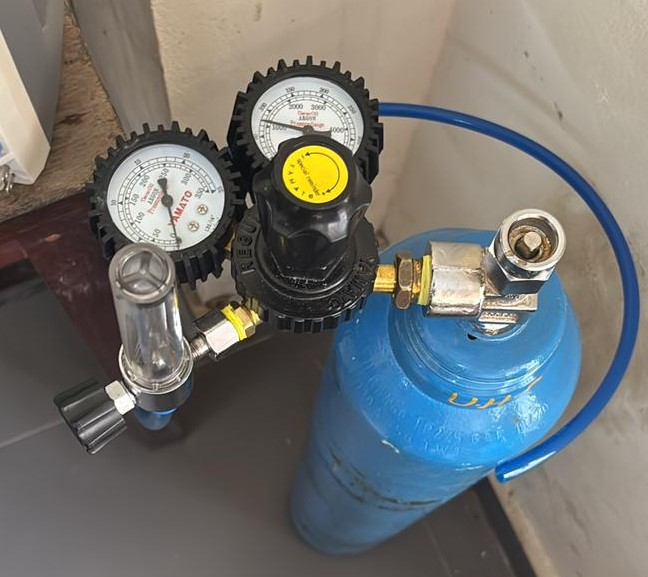
\includegraphics[width=\textwidth]{./picture-files/Hardware setup/top view.jpeg}
    \caption{Top view of the setup}
\end{subfigure}

\caption{Different views of the plasma generation setup.}
\label{fig:hardware_views}

\end{figure}

\section{Summary}

The hardware implementation of the cold plasma generation system was completed through iterative prototyping and PCB refinement. The final system consists of:
\begin{enumerate}
    \item UCC21330-based H-bridge inverter operating at 100~kHz  
    \item Multi-output power supply generating 320~V, 12~V, and 5~V DC  
    \item STM32G431-based controller with PWM generation and protection  
    \item Isolated voltage and current sensing module  
    \item ETD-59 high-frequency step-up transformer (14:170 turns ratio)  
    \item Resin-encapsulated Cockcroft--Walton multiplier ($\approx 30~\text{kV}$)  
    \item Argon-based plasma generation setup  
\end{enumerate}